\documentclass[11pt]{article}
\usepackage[margin=1in]{geometry}
\usepackage{graphicx}
\usepackage{booktabs}
\usepackage{amsmath}
\usepackage[hidelinks]{hyperref}
\usepackage{xcolor}
\usepackage{caption}
\captionsetup{font=small}

\title{Do Ray-Traced Cities Make a Better Channel Prior for an Unseen Site?\\[4pt]
\large A pre-registered study in simulation, and a test on measured channels that reverses it}
\author{Krish Patel}
\date{October 2026}

\begin{document}
\maketitle

\begin{abstract}
Channel estimators for a newly deployed base station are usually built from
3GPP stochastic channel models, which describe no particular street. Ray
tracers can simulate real city layouts instead. We ask whether a channel prior
built from many ray-traced cities serves an \emph{unseen} site better than one
built from 3GPP CDL models, and whether learned estimators are what make the
difference. Using Sionna RT on 14 city scenes (4 built-in, 10 generated from
OpenStreetMap), linear MMSE estimation from covariance priors, and
leave-one-city-out evaluation with outcomes and pass/fail bars written down
before each main experiment, we find in simulation that a covariance prior
pooled over many cities sits about 0.6\,dB from a site-trained estimator with
no site measurements---about what CDL reaches after 50 site measurements---and
that pooling acts as insurance against a badly matched source city. Learned
models added little: a CNN refiner gained at most 0.65\,dB in channel
estimation, and for channel prediction a simple per-user classical method beat
CNN predictors by 1.8--12\,dB at horizons of 2\,ms and beyond; a CNN trained to
correct the classical method added a repeatable 0.3--0.6\,dB. We then tested
the main simulation finding on measured channels from the DICHASUS outdoor
dataset (1.272\,GHz, three 2$\times$8 arrays on one building). There, the
pooled ray-traced prior was 3.2--4.1\,dB \emph{worse} than CDL on the full
array with no site data. The simulated channels were cleaner in delay than the
measured street; an exploratory rerun with diffuse scattering and diffraction
enabled in the ray tracer brought the ray-traced prior to within 0.3--0.5\,dB
of CDL, but placing the simulated users at the real users' distances undid
most of that (2.9\,dB behind CDL): the measured street carries multipath the
map-built scenes do not produce. All results are from one measured site and
one band.
\end{abstract}

\section{Introduction}

A base station estimates the radio channel to each user from a few pilot
symbols. Linear MMSE (LMMSE) estimation does this well when it knows the
channel's second-order statistics (its covariance across antennas, subcarriers
and time); learned estimators can in principle exploit more. At a new site,
neither the covariance nor training data is available, so estimators start from
a generic prior---typically the 3GPP CDL/TDL models of TR~38.901~\cite{tr38901}---and
adapt as site measurements arrive.

Differentiable ray tracers such as Sionna RT~\cite{sionnart} can simulate
propagation in real city geometry. Recent work uses ray-traced data as a
site-specific prior for a known site
\cite{delmoro2026,alikhani2025,abouamer2024}, pre-trains across source cities for
CSI feedback~\cite{sifo2026}, and compares stochastic with ray-traced data for
machine learning~\cite{morais2025}. We ask a narrower question: for a site
\emph{with no geometry model and no measurements}, is a prior pooled from
\emph{other} ray-traced cities better than the 3GPP models? And is a learned
estimator what makes the difference?

We answer in three steps: (i) leave-one-city-out experiments in simulation,
(ii) the same question for short-term channel prediction, where learning has
more room, and (iii) a test of the main simulation finding on measured
channels. Each main experiment's expected outcome and pass/fail bar was
committed to the lab notebook before it ran; follow-up checks are labelled as
post-hoc or exploratory. The code, notebook, logs and result tables are
available with the paper.

\section{Setup}

\paragraph{Grid and estimation.} A 5G NR-like OFDM slot: 3.5\,GHz carrier,
30\,kHz subcarrier spacing, 128 subcarriers $\times$ 14 symbols, DMRS-like
pilots on every other subcarrier of symbols 2 and 11, and an 8-antenna
half-wavelength uniform linear array at the base station. Channels are
normalised to unit power per sample. The estimator is LMMSE from a covariance
prior $(R_{hp}, R_{pp})$ estimated from 12k simulated channels. With $N$ site
measurements, the prior is shrunk toward their sample covariance with a weight
chosen by 5-fold cross-validation. A residual CNN (zero-initialised last layer,
so it starts at its LMMSE front end) tests whether anything beyond second-order
statistics helps. Error is NMSE at 10\,dB SNR unless stated, and the
``ceiling'' is LMMSE from 12k channels of the target site itself.

\paragraph{Channel sources.} All channels are generated with
Sionna~\cite{sionna}. \emph{CDL}: 3GPP CDL-A to E with delay spread
30--300\,ns and a random base-station heading per sample (a fixed heading made
CDL artificially poor in an early run, which we corrected and report).
\emph{Ray-traced (RT)}: Sionna RT~2.2 with up to 3 specular bounces and
refraction, in Sionna's four built-in scenes (Munich, Paris-\'Etoile, Florence,
San Francisco) and ten New York State areas built from OpenStreetMap with
geo2sigmap~\cite{geo2sigmap}, reading buildings from an offline Geofabrik
extract. Base stations are placed 25--40\,m up near the scene centre and users
within 250\,m.

\paragraph{Protocol.} Each city in turn is the unseen target; priors come from
the other cities (pooled with equal weight) or from CDL. Test users are at
base-station sites the priors never saw. The realism result was re-checked on
fresh base-station sites and freshly drawn pre-training sets.

\section{Results in simulation}

\paragraph{Ray-traced vs CDL, four cities.} With no site data, a prior pooled
from the three other built-in cities beat CDL in Munich (+0.3--0.5\,dB),
Florence (+1.1--1.2) and San Francisco (+1.3--1.5) and lost in \'Etoile
(--1.2 to --1.8) across the original and two fresh draws of sites and
pre-training data. The advantage faded with site data: by $N{=}1000$ all priors
were within $\sim$0.2\,dB except \'Etoile.

\paragraph{Fourteen cities: pooling as insurance.} Pooling $k$ random other
cities (8 draws each), the \emph{worst} draw's gap to the ceiling shrank from
3.99\,dB at $k{=}1$ to 0.82\,dB at $k{=}8$, while the average went from 1.59 to
0.60\,dB (Fig.~\ref{fig:breadth}): pooling protects against a badly matched
source city (the worst single-city cases, 6--7\,dB, all used a nearly empty
open-area scene as the source for a dense downtown). The all-cities pool beat
CDL in 11 of 14 targets by 0.29\,dB on average. With no site data it sat
0.59\,dB from the ceiling, about where CDL lands after 50 site measurements
(0.47--0.73\,dB across four draws of those 50). Once 50 measurements are
blended in, the two are comparable (pooled ahead by $\sim$0.1\,dB on built-up
sites). Choosing a single best source city from 50 measurements worked with 3
candidates (mean regret 0.05\,dB) but overfit with 15 (0.48\,dB, against a
pre-registered bar of 0.3).

\begin{figure}[t]
\centering
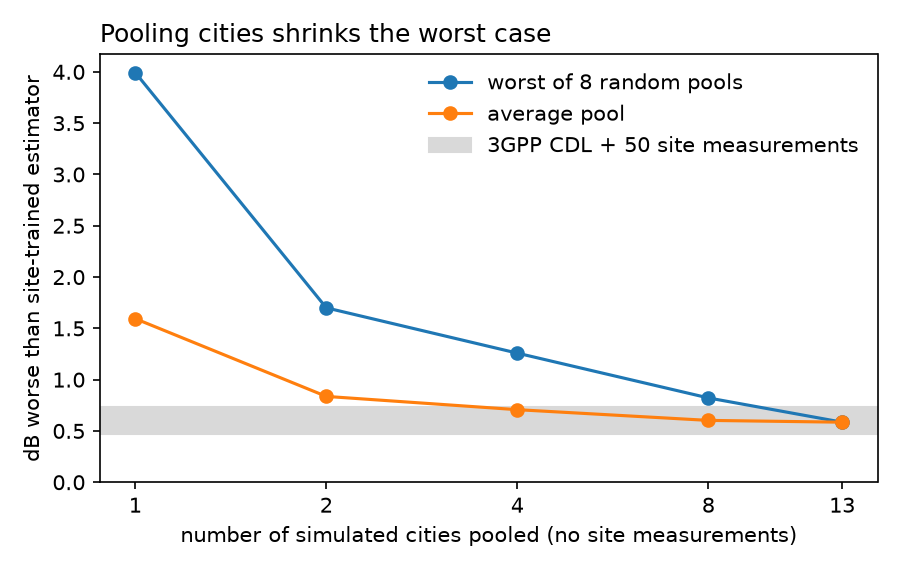
\includegraphics[width=0.68\linewidth]{../figures/breadth.png}
\caption{Simulation: gap to a site-trained estimator vs.\ the number of pooled
ray-traced cities, no site measurements, mean over 14 targets. The grey band is
3GPP CDL after blending in 50 site measurements.}
\label{fig:breadth}
\end{figure}

\paragraph{Learning in estimation.} The CNN refiner added $\sim$0.2--0.45\,dB
on the CDL prior and often nothing on ray-traced priors, at most 0.65\,dB in any
cell (one seed). The covariance did almost all of the work.

\section{Learning where it should have room: channel prediction}

Predicting the channel 0.5--10\,ms ahead from 1.4\,ms of noisy pilot history
(8 observations over 4 slots) is a task where per-user adaptation matters: a
covariance pooled over users cannot know each user's Doppler. Sionna RT
evolves a moving user by rotating the phases of a fixed set of paths; we
checked that this matches re-tracing at the moved position up to $\sim$10\,ms
for nearly all users at 3.5\,GHz (with the solver's deterministic mode), so we
restricted horizons to 10\,ms.

On 3GPP-compliant simulated channels, learned predictors have been reported to
beat a Prony-based angle--delay baseline~\cite{wifo}. We compared repeating the last observation, space-time Wiener prediction from
covariance priors, a classical per-user method (``tone'': in the angle--delay
domain, fit one Doppler tone per bin to the history and extrapolate), and CNN
predictors in the antenna and angle--delay domains. The pre-registered test for
``learning has room'' failed: tone beat both CNN arms at every horizon from
2\,ms in every city, by 1.8--4.7\,dB in Munich, \'Etoile and Florence and by
$\sim$9--12\,dB in San Francisco (Fig.~\ref{fig:pred}). The CNNs did beat
covariance-based prediction by 2--6\,dB at 2\,ms; learning was competitive only
one slot (0.5\,ms) ahead.

A post-hoc follow-up trained a CNN to \emph{correct} tone's prediction, with a
loss weighted toward the predictable horizons. It added 0.3--0.6\,dB at
2--10\,ms in three of four cities (cells 0.26--0.65; two seeds agree within
$\sim$0.2\,dB) and cost 0.8--1.2\,dB at 5--10\,ms in San Francisco, where tone is
already near-exact. Re-weighting the original CNNs' loss alone did not help.
The caveat that matters most: fixed-path evolution is tone's own model, so on
real channels tone would degrade by an amount this simulator cannot measure.

\begin{figure}[t]
\centering
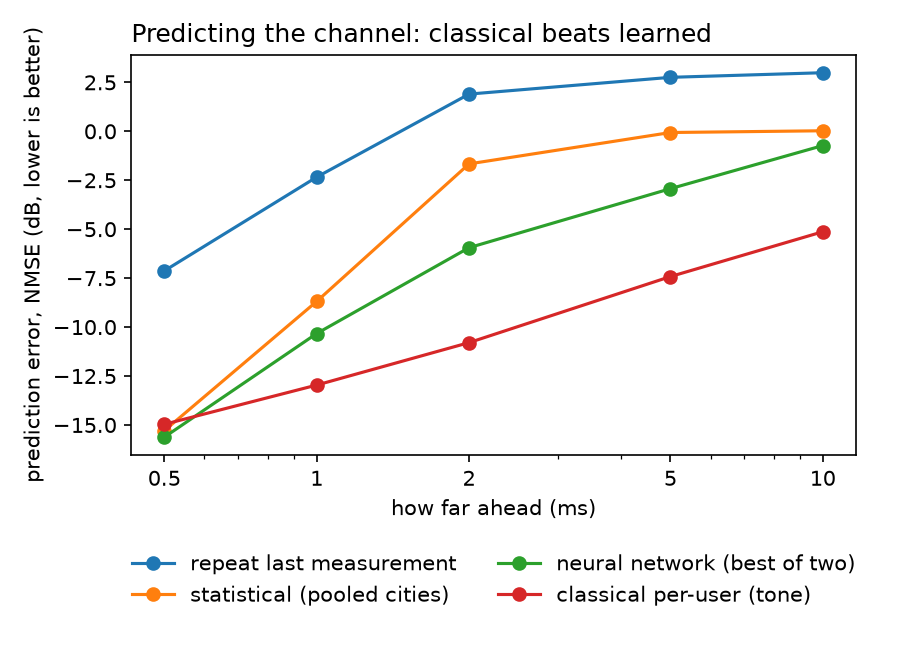
\includegraphics[width=0.68\linewidth]{../figures/prediction.png}
\caption{Simulation: prediction error vs.\ horizon, mean over four cities,
10\,dB SNR, no site data. ``Neural network'' is the better of the two CNN arms
in each cell.}
\label{fig:pred}
\end{figure}

\section{Test on measured channels}

\paragraph{Data.} DICHASUS~\cite{dichasus} outdoor set \texttt{dxxx}
\cite{dichasusdata}: three 2$\times$8 arrays ($\lambda/2$ at 1.272\,GHz) on one
building facade about 10\,m up and tilted $\sim$20$^\circ$ down, a hand-pulled
transmitter on the street, 50\,MHz over 1024 subcarriers, tachymeter
positions. Calibration files (also used for the ceiling), a site file (50
random measurements, 4 draws) and test files are disjoint recordings.

\paragraph{Processing.} The receivers carry constant per-antenna phase and
timing offsets, as the dataset authors describe; offset files are not shipped
for this set. We fit, per antenna, a phase plus a delay relative to a reference
antenna to the line-of-sight phase predicted from the tachymeter positions;
the fit also identified the array layout (8-element axis horizontal: coherence
0.73 on array A versus at most 0.32 for the alternative layouts in an early fit;
0.80 on the full calibration set).
Every source---measured, CDL and ray-traced---is generated on the full
50\,MHz band and passes through one chain: align the first arrival to delay
zero, keep a delay window of $-$200\,ns to 2\,$\mu$s, take the 128 subcarriers
around the carrier (6.25\,MHz), normalise. The grid is 16 antennas $\times$ 128
subcarriers in one snapshot, pilots on every other subcarrier. All 14 cities
were re-simulated at 1.272\,GHz with the 2$\times$8 array, a directional
38.901 element pattern, a 20$^\circ$ downtilt and a facade-like placement
(base station 10\,m above ground, users 10--65\,m in front, outdoor positions
only, heights following terrain).

\paragraph{Results.} The pre-registered claim that the pooled ray-traced prior
beats CDL with no site data was falsified on all three arrays
(Table~\ref{tab:measured}, Fig.~\ref{fig:measured}): it was 3.2--4.1\,dB worse
on the full array $\times$ frequency grid and 0.5--1.3\,dB worse per antenna.
On the full grid no single city beat CDL either. With 50 site measurements CDL
still led by 1.2--1.7\,dB on the full grid; per antenna both reached the
site-trained level. Pooling still shrank the worst single-city case in 5 of 6
checks, but around a level below CDL. The pool sat 5.8--6.8\,dB from the
ceiling, against $\sim$0.6\,dB in simulation.

\begin{table}[t]
\centering
\small
\begin{tabular}{lrrrrr}
\toprule
array & LS interp. & CDL & RT pool (specular) & RT pool (scattering) & ceiling \\
\midrule
A & $-$11.2 & $-$17.9 & $-$14.7 & $-$17.6 & $-$20.5 \\
B & $-$11.2 & $-$17.5 & $-$13.4 & $-$17.0 & $-$20.2 \\
C & $-$11.2 & $-$17.9 & $-$14.4 & $-$17.5 & $-$20.4 \\
\bottomrule
\end{tabular}
\caption{Measured DICHASUS channels: NMSE (dB) at 10\,dB SNR on the full
16-antenna $\times$ 128-subcarrier grid, no site measurements. Specular pool:
14 cities; scattering pool: 7 cities (exploratory).}
\label{tab:measured}
\end{table}

\begin{figure}[t]
\centering
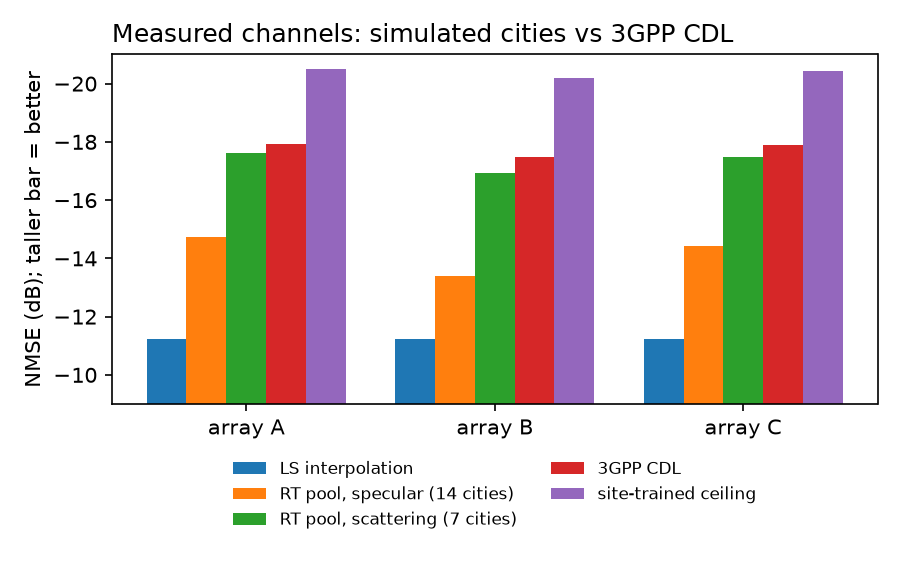
\includegraphics[width=0.68\linewidth]{../figures/measured.png}
\caption{Measured channels, the same numbers as Table~\ref{tab:measured}.}
\label{fig:measured}
\end{figure}

\paragraph{Why.} The simulated channels were cleaner in delay than the
measured street: 89--100\% of energy in the first 160\,ns tap across the 14
cities, against 79--84\% measured (CDL 79\%). Spatial concentration was not
clearly different. The ray tracer ran with the original study's settings:
specular reflection and refraction only, no diffuse scattering, no diffraction,
every material's scattering coefficient zero. In an exploratory rerun, added
after a dry run and labelled as such, we enabled diffuse scattering
(coefficient 0.3, Lambertian) and Sionna's wedge diffraction for 7 cities.
The pooled prior came within 0.3--0.5\,dB of CDL on the full grid and level
with it per antenna. A control with the same cities and the same number of
base-station sites but no scattering attributes $\sim$2.8\,dB of the
$\sim$3\,dB improvement on array A to scattering and diffraction and
$\sim$0.2\,dB to the extra sites.

\paragraph{Matching the users' distance made it worse.} The simulated users
sat farther from the array than the real ones (median 46\,m vs 18--20\,m). In a
second exploratory probe, with scattering on and users placed 12--30\,m away,
the ray-traced prior fell to 2.9\,dB behind CDL on array A (2.1--2.6\,dB worse
than the farther placement on every array and grid). Closer simulated users
are more line-of-sight dominated (first-tap share 89--97\%), while the real
users at those distances show 79--84\%: the measured street has multipath
the map-built scenes do not produce, plausibly from objects they lack
(vehicles, trees, street furniture, facade detail). The near-match of the
scattering variant therefore came partly from placing users farther away than
the real ones.


\section{Discussion and limitations}

The simulation finding was a home-ground effect, as the caveat written before
the first run anticipated: test channels came from the same ray tracer as the
priors. CDL is fitted to measurements; ray tracing at default settings encodes
geometry but misses diffuse multipath, and every ray-traced candidate is biased
the same way, so pooling cannot insure against it. Several limits apply.
\begin{itemize}
\item One measured site: one street, one building, three arrays on its
  facade, 1.272\,GHz, mostly line-of-sight; LMMSE estimation only.
\item The measured-channel test was pre-registered but not blind: a pilot had
  already scored CDL on the test data, and a dry run preceded the full run.
\item The simulated placement was not matched to the real users (median 46\,m
  and $\sim$10$^\circ$ below the array by the placement rule, versus
  18--20\,m and 24--26$^\circ$ measured), and one downtilt was used for all
  three arrays.
\item Small asymmetries remain: measured channels sit $\sim$10--20\,ns later
  after alignment than simulated ones (bounded at $\sim$0.5\,dB of the
  CDL-vs-pool gap), and the correlation between the two antenna rows is lower
  in the measured data than in either model, for reasons not established.
\item Most randomly placed users in the rooftop simulations received no paths
  and were dropped, so simulated users skew toward simpler links.
\item The scattering result uses one scattering value and 7 cities, and was
  chosen after seeing the dry run; matching the users' distance undid most of
  it.
\end{itemize}
A code review during the measured-channel work found a cache keyed on object
identity that could hand a scene another scene's ground mesh; it was fixed and
everything rerun, and reported numbers moved by at most 0.02\,dB.

\section{Conclusion}

In simulation, a covariance prior pooled over many ray-traced cities looked
like a good starting point for an unseen site and a safer one than any single
city. On measured channels from one site, it was worse than the 3GPP CDL
models, because the simulated channels were too clean; with diffuse scattering
and diffraction enabled it roughly matched CDL, but only with users placed
farther away than the real ones. Learned models never beat the
classical methods; at best they refined them. For a ray-traced prior to be
useful at a real site, the simulator's settings matter at least as much as the
number of cities.

\paragraph{Where next.} Three directions follow from the results.
(i) \emph{Tune the simulator, not the covariance, from site measurements:}
the gap is driven by global simulator settings and missing scene content, so a
few site measurements could set the scattering level (or a clutter model) that
is then used to simulate other cities, with no 3D model of the target site.
Existing calibration work tunes a single, fully modelled site
\cite{hoydis2023learning}; a coarse grid over the scattering coefficient,
scored on 50 site measurements, is a cheap first test. (ii) \emph{More
measured sites}, since one street cannot settle a question about unseen
sites; we found no public outdoor dataset with several sites and a planar
array. (iii) \emph{Prediction on measured channels}, where the classical
method's advantage rests on a simulator that matches its own model; this needs
millisecond-spaced measurements of moving users.

\paragraph{Reproducibility.} Code, the lab notebook with every
pre-registration and result in order, logs and result tables accompany the
paper. Channel sets are regenerated by the scripts; the measured data is
public under CC BY 4.0~\cite{dichasusdata}.

\begin{thebibliography}{99}\small
\bibitem{tr38901} 3GPP, ``Study on channel model for frequencies from 0.5 to 100 GHz,'' TR 38.901.
\bibitem{sionna} J.~Hoydis, S.~Cammerer, F.~Ait~Aoudia, A.~Vem, N.~Binder, G.~Marcus, A.~Keller, ``Sionna: An open-source library for next-generation physical layer research,'' arXiv:2203.11854, 2022.
\bibitem{sionnart} J.~Hoydis, F.~A\"it~Aoudia, S.~Cammerer, M.~Nimier-David, N.~Binder, G.~Marcus, A.~Keller, ``Sionna RT: Differentiable ray tracing for radio propagation modeling,'' arXiv:2303.11103, 2023.
\bibitem{geo2sigmap} Functions Lab, ``geo2sigmap,'' \url{https://github.com/functions-lab/geo2sigmap} (commit 08ca016).
\bibitem{dichasus} F.~Euchner, M.~Gauger, S.~D\"orner, S.~ten~Brink, ``A distributed massive MIMO channel sounder for `big CSI data'-driven machine learning,'' WSA 2021; arXiv:2206.15302.
\bibitem{dichasusdata} University of Stuttgart, ``CSI dataset dichasus-dxxx-complete: Outdoor---three arrays distributed along the facade,'' DaRUS, doi:10.18419/DARUS-3153, CC BY 4.0.
\bibitem{delmoro2026} L.~Del~Moro \emph{et al.}, ``Site geometry and calibration uncertainties in digital twin-enabled channel estimation,'' arXiv:2607.09334, 2026.
\bibitem{alikhani2025} S.~Alikhani \emph{et al.}, ``Digital twin aided channel estimation: Zone-specific subspace prediction and calibration,'' arXiv:2501.02758, 2025.
\bibitem{abouamer2024} M.~S.~Abouamer \emph{et al.}, ``Prediction of wireless channel statistics with ray tracing and uncalibrated digital twin,'' arXiv:2411.13360, 2024.
\bibitem{sifo2026} C.-J.~Zhao \emph{et al.}, ``SiFo: Wireless foundation model for low-overhead site-specific CSI feedback,'' arXiv:2605.16141, 2026.
\bibitem{wifo} B.~Liu \emph{et al.}, ``WiFo: Wireless foundation model for channel prediction,'' arXiv:2412.08908, 2024.
\bibitem{hoydis2023learning} J.~Hoydis, F.~A\"it~Aoudia, S.~Cammerer, F.~Euchner, M.~Nimier-David, S.~ten~Brink, A.~Keller, ``Learning radio environments by differentiable ray tracing,'' arXiv:2311.18558, 2023.
\bibitem{morais2025} J.~Morais, A.~Malhotra, S.~Hamidi-Rad, A.~Alkhateeb, ``Comparing stochastic and ray-tracing datasets in machine learning for wireless applications,'' arXiv:2512.12449, 2025.
\end{thebibliography}

\end{document}
